\documentclass[colorlinks]{thesis-kando}

% 1. PDF verzió kezelése (a figyelmeztetés megszüntetéséhez)
\pdfminorversion=7

% 2. Magyar nyelv specifikus beállítások (a babel ELŐTT)
\PassOptionsToPackage{defaults=hu-min}{magyar.ldf}

% 3. Alapvető kódolás és nyelvi csomag
\usepackage[T1]{fontenc}
\usepackage[utf8]{inputenc}
\usepackage[magyar]{babel}

% 4. Minden egyéb csomag duplikáció nélkül
\usepackage{graphicx,amsmath,amssymb,amsthm,hulipsum,bussproofs}
\usepackage{listings,xcolor,rotating,booktabs,fancyvrb}
\usepackage[normalem]{ulem}
\usepackage{pdfpages}
\usepackage[linguistics]{forest}
\usepackage{stackengine,scalerel}
\usepackage{url}
\def\UrlBreaks{\do\/\do-\do\.\do\a\do\b\do\c\do\d\do\e\do\f\do\g\do\h\do\i\do\j\do\k\do\l\do\m\do\n\do\o\do\p\do\q\do\r\do\s\do\t\do\u\do\v\do\w\do\x\do\y\do\z\do\0\do\1\do\2\do\3\do\4\do\5\do\6\do\7\do\8\do\9}
% Formázási és matematikai beállítások
\footnotestyle{rule=fourth}
\DeclareMathOperator{\tg}{tg}
\newtheorem{tetel}{Tétel}[chapter]
\newtheorem{lemma}[tetel]{Lemma}
\theoremstyle{definition}
\newtheorem{definicio}[tetel]{Definíció}
\newtheorem{feladat}[tetel]{Feladat}
\theoremstyle{remark}
\newtheorem{megjegyzes}[tetel]{Megjegyzés}
\newtheorem*{megoldas}{Megoldás}

% Listings beállítása a magyar karakterekhez
\lstset{
	inputencoding=utf8,
	extendedchars=true,
    literate={á}{{\'a}}1 {é}{{\'e}}1 {í}{{\'i}}1 {ó}{{\'o}}1 {ö}{{\"o}}1 {ő}{{\H{o}}}1
    {ú}{{\'u}}1 {ü}{{\"u}}1 {ű}{{\H{u}}}1
    {Á}{{\'A}}1 {É}{{\'E}}1 {Í}{{\'I}}1 {Ó}{{\'O}}1 {Ö}{{\"O}}1 {Ő}{{\H{O}}}1
    {Ú}{{\'U}}1 {Ü}{{\"U}}1 {Ű}{{\H{U}}}1,
    breaklines=true,
    basicstyle=\ttfamily\small,
    keywordstyle=\color{blue},
    commentstyle=\color{gray},
    stringstyle=\color{teal}
}


% Define JavaScript language for listings
\lstdefinelanguage{JavaScript}{
    keywords={break, case, catch, continue, debugger, default, delete, do, else, finally, for, function, if, in, instanceof, new, return, switch, this, throw, try, typeof, var, void, while, with, let, const, export, import, await, async},
    ndkeywords={class, export, boolean, throw, implements, import, this, new},
    sensitive=true,
    comment=[l]{//},
    morecomment=[s]{/*}{*/},
    morestring=[b]',
    morestring=[b]",
    alsoletter={-},
    alsodigit={:},
    morekeywords=[2]{=>, yield, async, await, constructor},
    keywordstyle=\color{blue}\bfseries,
    ndkeywordstyle=\color{green}\bfseries,
    identifierstyle=\color{black},
    commentstyle=\color{gray}\ttfamily,
    stringstyle=\color{red}\ttfamily,
}

% Customize listings appearance
\lstset{
    language=JavaScript,
    extendedchars=true,
    inputencoding=utf8,
    basicstyle=\ttfamily\small,
    numbers=left,
    numberstyle=\tiny\color{gray},
    stepnumber=1,
    numbersep=10pt,
    showstringspaces=false,
    breaklines=true,
    frame=single,
    captionpos=b,
    escapeinside={\%*}{*)},
}

% Fordított 'T' szimbólum definiálása
\def\tang{\ThisStyle{\abovebaseline[0pt]{\scalebox{-1}{$\SavedStyle\perp$}}}}

\begin{document}

\title{Project Hephaistos}

\author{Barna Bence\\Fehér Valentin\\Fekete Dávid\\Szoftverfejlesztő és -tesztelő szak}
\institute{Informatika és távközlés ágazat}
\supervisor{Kerényi Róbert Nándor\\oktató}
\city{Miskolc}
\date{2025}
\begin{figure}[h]
    \centering
    \label{fig:minta}
\end{figure}
\maketitle

\tableofcontents
\newpage

% --- 1. fejezet ---
\chapter{Bevezetés}
\section{A projekt bemutatása és célja}
% --- Kép beszúrása ---
Kép beszúrása
\begin{figure}[ht!]
	\centering
	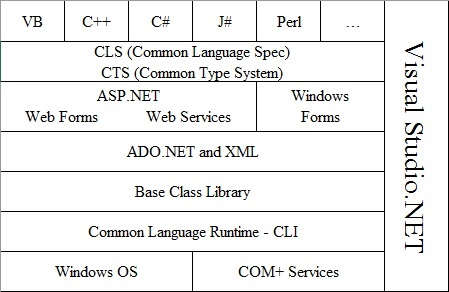
\includegraphics[width=9cm]{figures/dotNET}
	\caption[dotNET]{.NET keretrendszer}
	\label{fig-dotNET}
\end{figure}

\section{Célközönség meghatározása}
Forrásmegjelölés
\newline
Az automatikus tételbizonyítás egyik fontos megközelítése Herbrand nevéhez fűződik (1930). Herbrand algoritmust dolgozott ki olyan interpretáció előállítására, amely hamissá tehet egy formulát. Ugyanakkor, ha az illető formula logikailag igaz, tehát nincs olyan interpretáció, amelyben hamissá válna, ez az algoritmus véges sok lépés után megáll. {\cite{Varteresz}}
\section{Alkalmazott technológiák és eszközök}
Mellékletre hivatkozás:
\newline
 Lásd: \ref{fig-melleklet1} melléklet ábrát. 
\begin{itemize}
	\item \textbf{Adatbázis:} MySQL
	\item \textbf{Backend:} RESTful API (pl. ASP.NET Core / Node.js)
	\item \textbf{Webes kliens:} React (Reszponzív kialakítás)
	\item \textbf{Asztali kliens:} WPF (C\#)
\end{itemize}
\newline
Táblázat
\newline
\begin{table}[ht]
	\centering
	\begin{tabular}{lll}
		\hline
		\multicolumn{1}{|l|}{\textbf{SZIMBÓLUM}} & \multicolumn{1}{l|}{\textbf{MAGYAR MEGNEVEZÉS}} & \multicolumn{1}{l|}{\textbf{IDEGEN MEGNEVEZÉS}} \\ \hline
		\multicolumn{1}{|l|}{\boldmath$\land$} & \multicolumn{1}{l|}{\textbf{ÉS}} & \multicolumn{1}{l|}{\textbf{KONJUNKCIÓ}} \\ \hline
		\multicolumn{1}{|l|}{\boldmath$\lor$} & \multicolumn{1}{l|}{\textbf{VAGY}} & \multicolumn{1}{l|}{\textbf{DISZJUNKCIÓ}} \\ \hline
		\multicolumn{1}{|l|}{\boldmath$\Rightarrow$} & \multicolumn{1}{l|}{\textbf{AKKOR..HA}} & \multicolumn{1}{l|}{\textbf{IMPLIKÁCIÓ}} \\ \hline
		\multicolumn{1}{|l|}{\boldmath$\Leftrightarrow$} & \multicolumn{1}{l|}{\textbf{AKKOR ÉS CSAK AKKOR}} & \multicolumn{1}{l|}{\textbf{EKVIVALENCIA}} \\ \hline
	\end{tabular}
\end{table}
% --- 2. fejezet ---
\chapter{Követelményanalízis}
\section{Funkcionális követelmények}
\section{Nem funkcionális követelmények}
\section{Használati esetek (Use Cases)}

% --- 3. fejezet ---
\chapter{Rendszertervezés}
\section{Adatbázis terv}
\subsection{ER-diagram és kapcsolatok}
\subsection{Adatszótár és táblaleírások}
\section{Rendszerarchitektúra és komponensek}
\subsection{ORM (Object-Relational Mapping)}
\subsection{Entity Framework}
\section{REST API végpontok tervezése}
\section{UI/UX Tervek (Wireframes)}

% --- 4. fejezet ---
\chapter{Megvalósítás}
\section{Adatbázis réteg implementációja}
\section{REST Backend fejlesztése}
\subsection{Adatkezelés és Üzleti logika}
\subsection{Biztonság és Autentikáció (JWT)}
\section{React Frontend fejlesztése}
\subsection{Komponens-architektúra}
\subsection{Reszponzív megoldások és Mobil nézet}
\section{WPF Desktop alkalmazás}
\subsection{MVVM architektúra és Adatkötés}
\subsection{Törzsadat-karbantartó modulok}

% --- 5. fejezet ---
\chapter{Minőségbiztosítás és Tesztelés}
\section{Unit tesztek (Egységtesztelés)}
\section{API tesztelés (Postman/Swagger)}
\section{Felhasználói felület és Reszponzivitás tesztelése}
\section{Hibajegyzék és javítások}

% --- 6. fejezet ---
\chapter{Felhasználói útmutató}
\section{Rendszerkövetelmények és Telepítés}
\section{A szoftver használata (Web/WPF)}

% --- 7. fejezet ---
\chapter{Összegzés}
\section{Projekt értékelése}
\section{Továbbfejlesztési lehetőségek}

\newpage
\Huge\begin{center}
    \textbf{Köszönetnyilvánítás}
\end{center}\normalsize
Szeretnék köszönetet mondani mindazoknak, akik segítették a vizsgaremekem létrejöttét, külön megköszönve.......
\par

\chapter{Vázrajz, ER diagram, brainstorming board}

\begin{figure}[ht!]
	\centering
	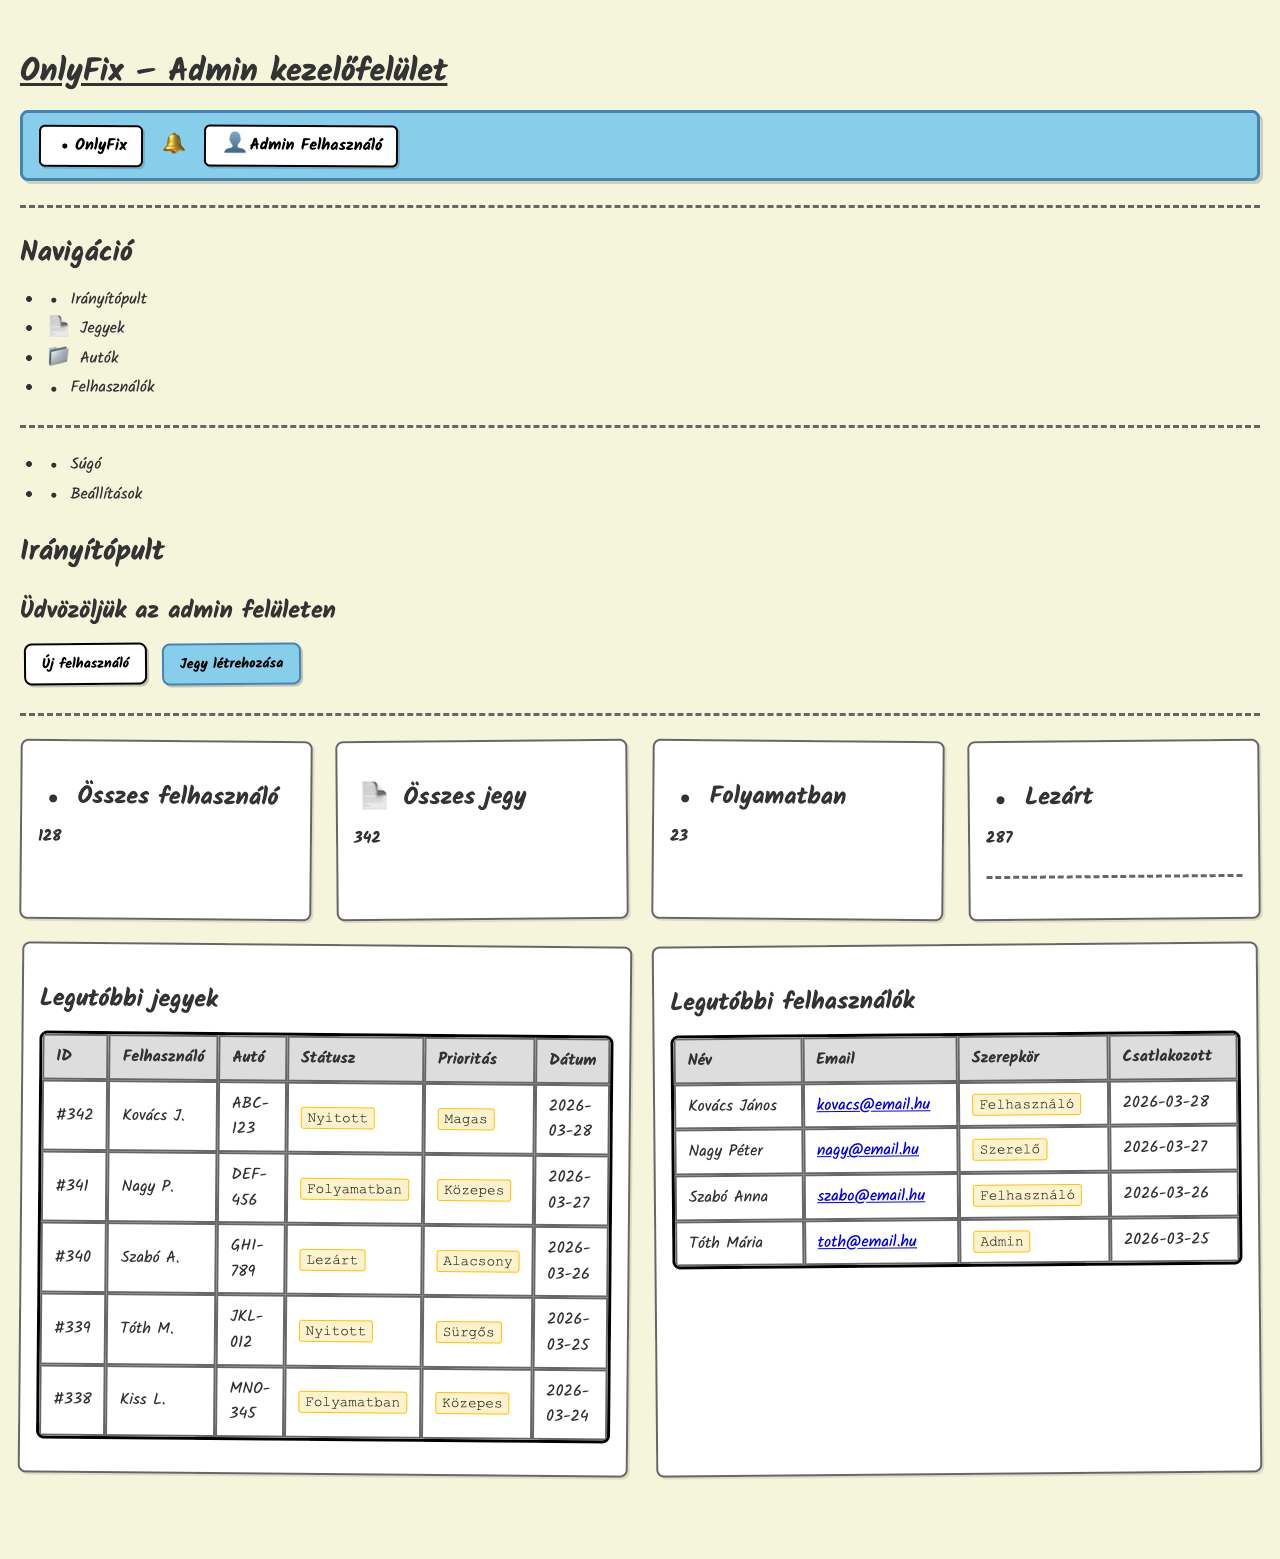
\includegraphics[width=13cm]{figures/03-admin-dashboard}
	\caption{Admin kezelőfelület vázrajz}
	\label{fig:figure1}
\end{figure}

\clearpage

\begin{figure}[ht!]
	\centering
	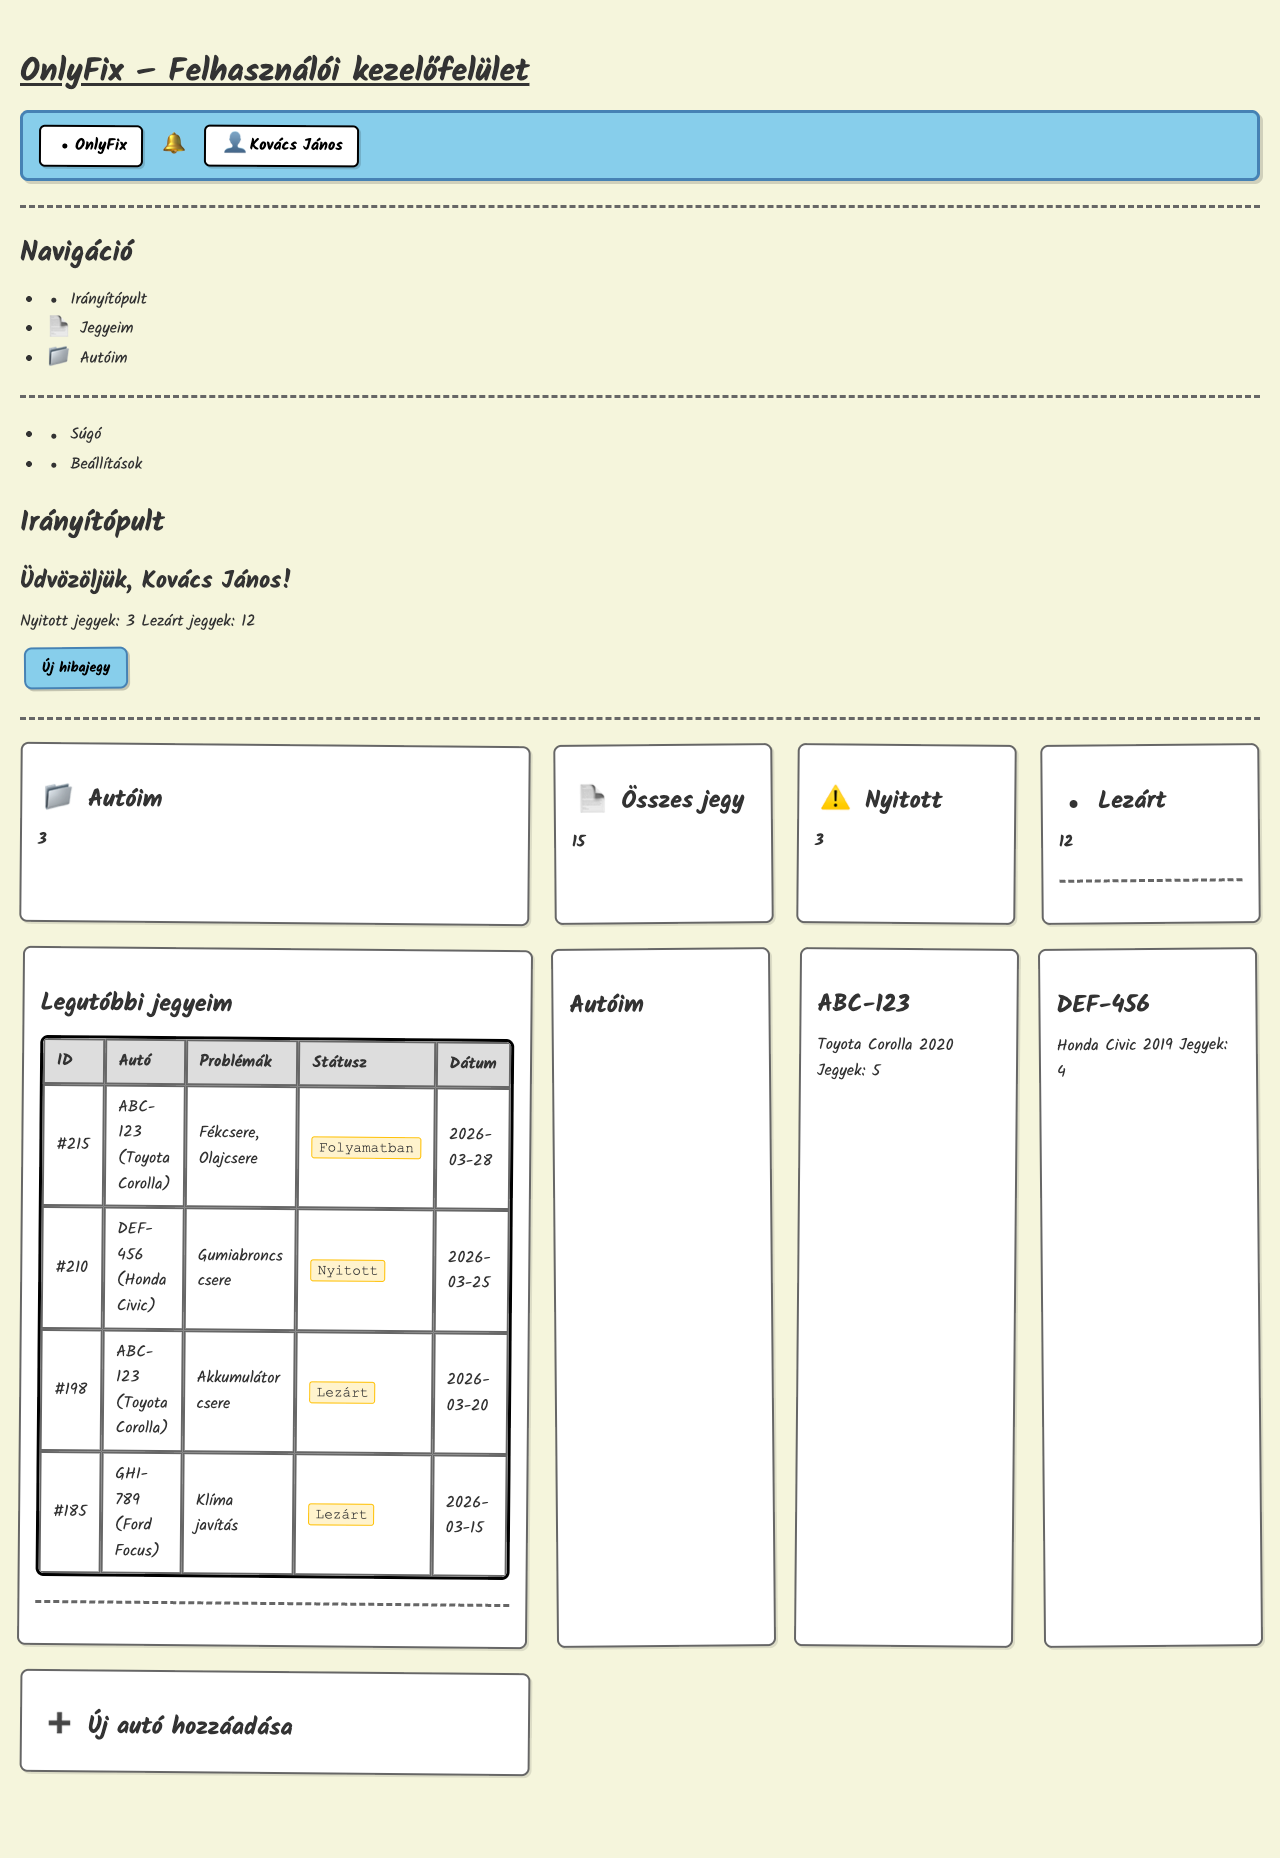
\includegraphics[width=13cm]{figures/04-user-dashboard}
	\caption{Felhasználói kezelőfelület vázrajz}
	\label{fig:figure2}
\end{figure}

\clearpage

\begin{figure}[ht!]
	\centering
	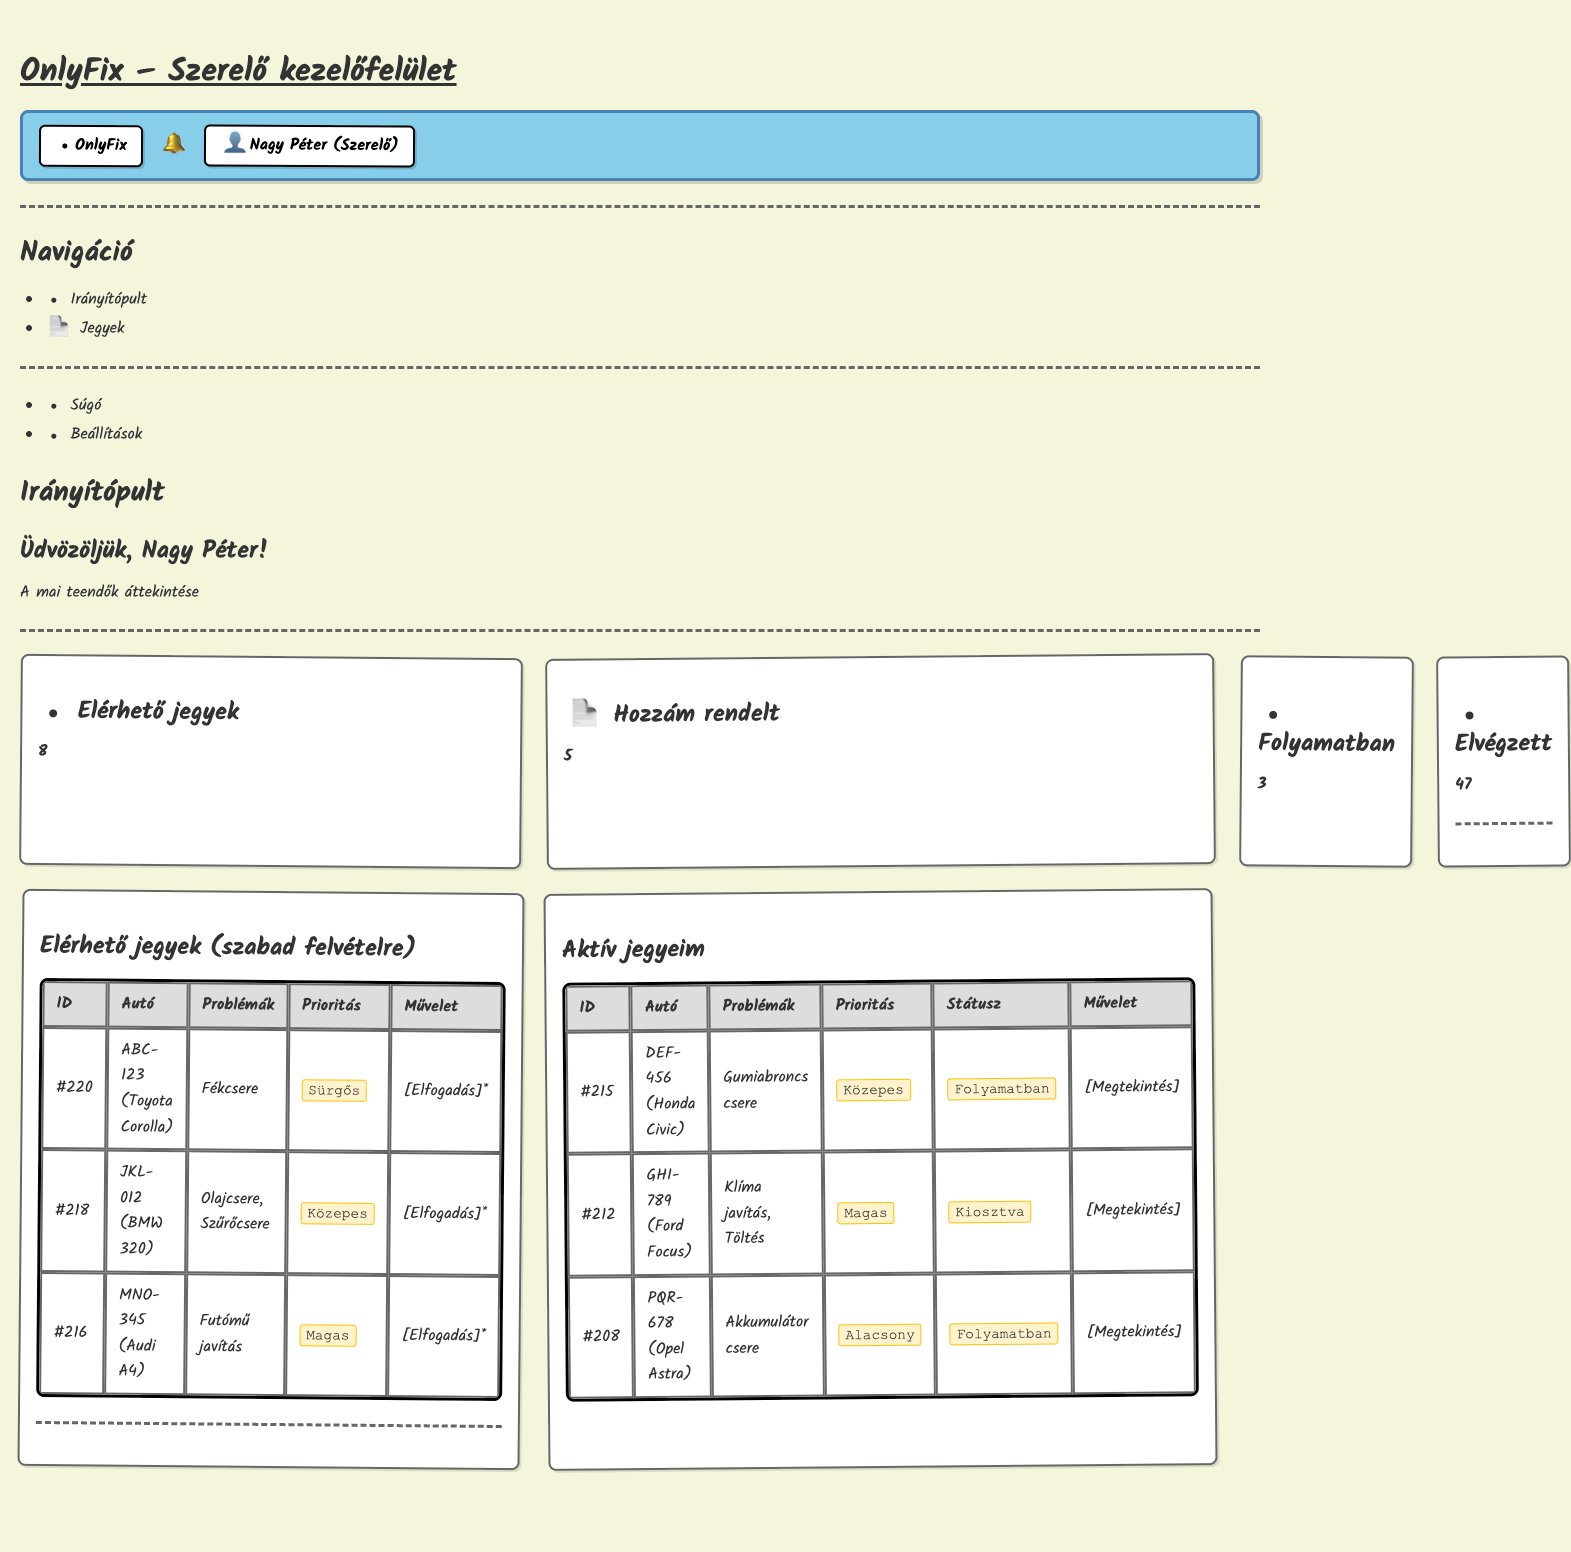
\includegraphics[width=13cm]{figures/05-mechanic-dashboard}
	\caption{Szerelői kezelőfelület vázrajz}
	\label{fig:figure3}
\end{figure}

\clearpage

\begin{figure}[ht!]
	\centering
	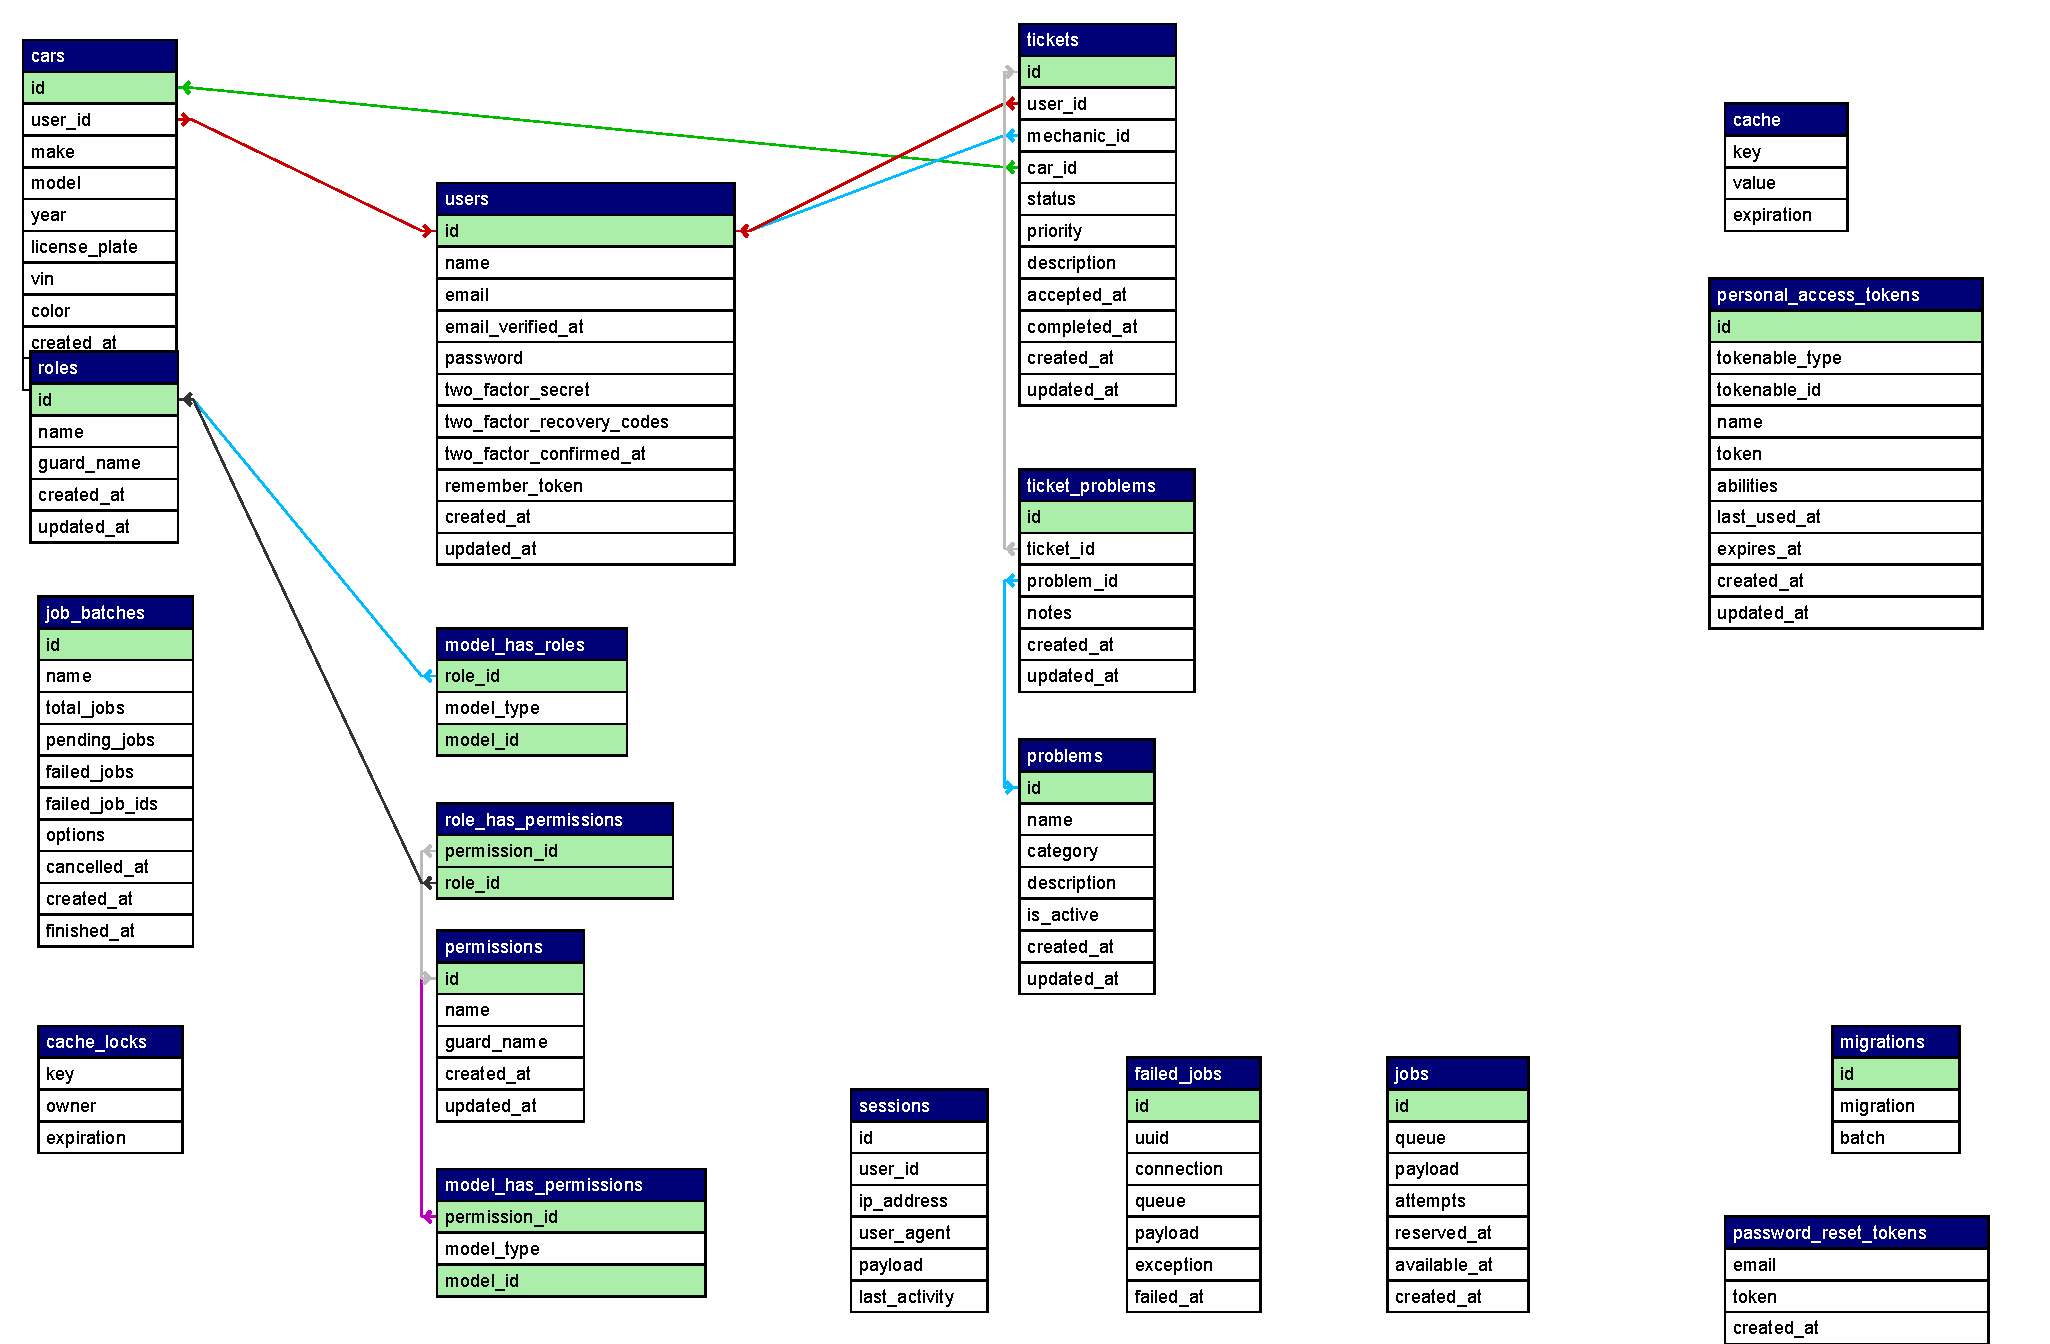
\includegraphics[width=14cm]{figures/onlyfix}
	\caption{ER diagram -- adatbázis séma}
	\label{fig:figure4}
\end{figure}

\clearpage

\begin{figure}[ht!]
	\centering
	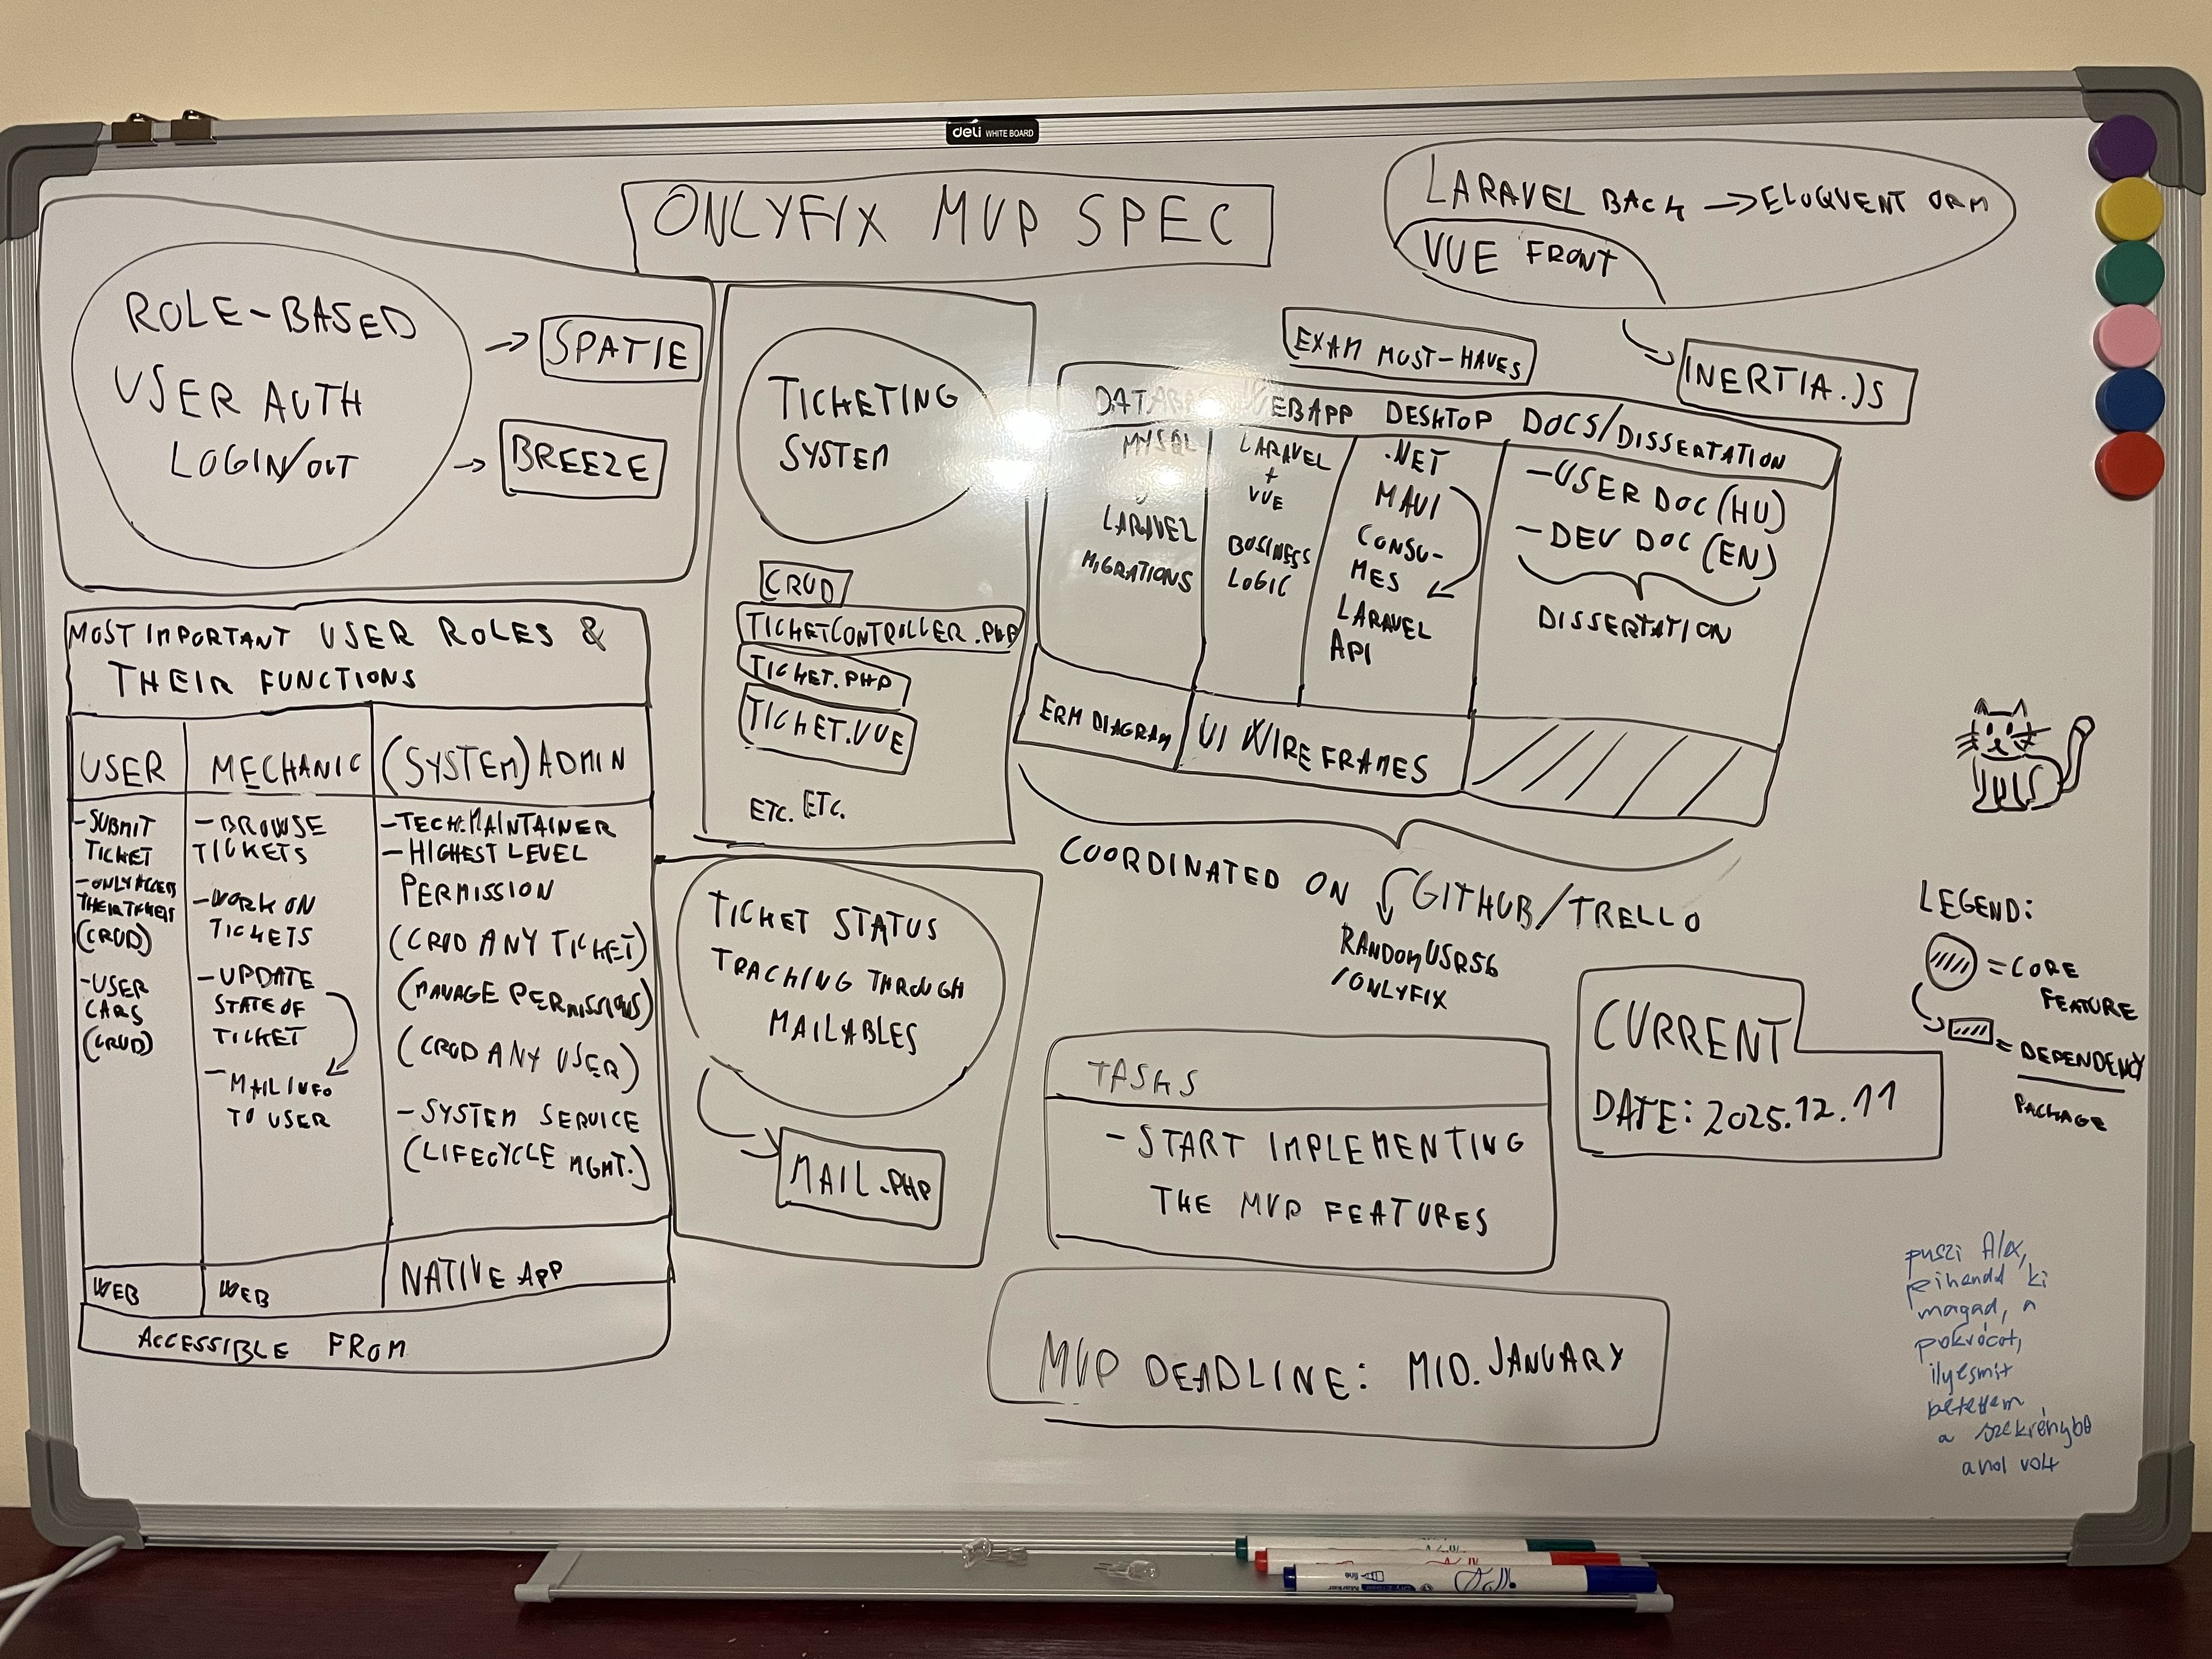
\includegraphics[width=14cm]{figures/mvp_specification}
	\caption{MVP specifikáció -- brainstorming board}
	\label{fig:figure5}
\end{figure}

\clearpage

\chapter*{Mellékletek}
\addcontentsline{toc}{chapter}{Mellékletek} % Hogy benne legyen a tartalomjegyzékben

% --- ELSŐ MELLÉKLET (Adatbázis) ---
\begin{figure}[ht!]
	\centering
	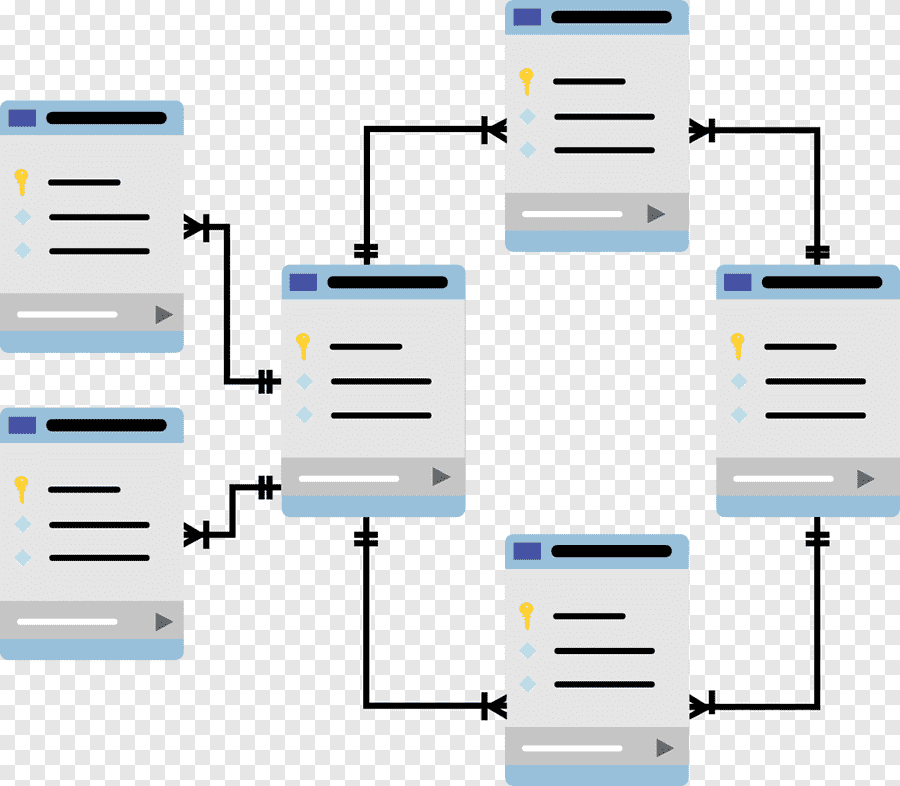
\includegraphics[width=14cm]{figures/rdb}
	\caption[1. melléklet]{Adatbázis ábra}
	\label{fig-melleklet1}
\end{figure}

\clearpage % Kényszerített oldalváltás a két melléklet között

% --- MÁSODIK MELLÉKLET (Elforgatott dokumentum) ---
\begin{figure}[p] % [p] = külön oldalra kerül
	\centering
	\begin{turn}{90}
		
\includegraphics[width=23cm]{figures/melleklet}
	\end{turn}
	\caption[2. melléklet]{Szkennelt dokumentum}
	\label{fig-melleklet2}
\end{figure}

\clearpage

\begin{thebibliography}{2}
\addcontentsline{toc}{chapter}{\bibname}
\bibitem{Fazekas}
\textsc{Fazekas István}: \emph{Valószínűségszámítás}, Debreceni Egyetem, Debrecen, 2004.
\bibitem{Tomacs}
\textsc{Tómács Tibor}: \emph{A valószínűségszámítás alapjai}, Líceum Kiadó, Eger, 2005.
\bibitem{Varteresz} \textsc{Várterész Magdolna}: \emph{Az informatika logika alapjai előadások}, 2006/07-es tanév 1.félév, \url{http://users.atw.hu/de-mi/index.php?r=file/download\&id=219},  Letöltve: 2019 március 12.-én
\end{thebibliography}


\end{document}

